%%%%%%%%%%%%%%%%%%%%%%%%%%%%%%%%%%%%%%%%%%%%%%%%%%%%
%%%                                              %%%
%%%     Language Science Press Master File       %%%
%%%         follow the instructions below        %%%
%%%                                              %%%
%%%%%%%%%%%%%%%%%%%%%%%%%%%%%%%%%%%%%%%%%%%%%%%%%%%%
 
% Everything following a % is ignored
% Some lines start with %. Remove the % to include them

\documentclass[output=long             % long|short|inprep              
% 	        ,blackandwhite
% 		,smallfont
%  	        ,draftmode  
		,biblatex
		  ]{LSP/langsci}    
  
%%%%%%%%%%%%%%%%%%%%%%%%%%%%%%%%%%%%%%%%%%%%%%%%%%%%
%%%                                              %%%
%%%          additional packages                 %%%
%%%                                              %%%
%%%%%%%%%%%%%%%%%%%%%%%%%%%%%%%%%%%%%%%%%%%%%%%%%%%%

% put all additional commands you need in the 
% following files. If you do not know what this might 
% mean, you can safely ignore this section

%%%%%%%%%%%%%%%%%%%%%%%%%%%%%%%%%%%%%%%%%%%%%%%%%%%%
%%%                                              %%%
%%%                 Metadata                     %%%
%%%          fill in as appropriate              %%%
%%%                                              %%%
%%%%%%%%%%%%%%%%%%%%%%%%%%%%%%%%%%%%%%%%%%%%%%%%%%%%

\title{Roots of Language}  %look no further, you can change those things right here.
% \renewcommand{\subtitle}{History and typology}
\BackTitle{Roots of Language} % Change if BackTitle != Title
\BackBody{}
\dedication{\parbox[t]{\textwidth}{\begin{flushleft}
	\textit{To the people of Palmares,\\
		\hspace{4em}El Palenque de San Basilio,\\
		\hspace{4em}The Cockpit Country,\\
		\hspace{4em}and the Saramacca River,\\
		who fought for decency, dignity, and freedom\\
		against the Cartesian savagery of Western colonialists\\
		\hspace{2em}and slavemakers;\\
		whose tongues, having survived\\		
		to confound pedagogue and philosopher alike,\\
		now, by an ironic stroke of justice,\\		
		offer us indispensable keys to the knowledge of\\
		\hspace{2em}our species.}		\end{flushleft}}
	}
%\typesetter{Change typesetter in localmetadata.tex}
%\proofreader{Change proofreaders in localmetadata.tex}
\author{Derek Bickerton}
\newlength{\csspine} 
\newlength{\bodspine}
\setlength{\csspine}{27.0559784mm} % Please calculate: Total Page Number (excluding cover, usually (Total Page - 3)) * 0.0572008 mm
\setlength{\bodspine}{40mm} % Please calculate: Total Page Number (excluding cover) * BODFACTOR + BODABS

\renewcommand{\lsISBNdigital}{978-3-946234-08-1}
\renewcommand{\lsISBNhardcover}{978-3-946234-09-8}
\renewcommand{\lsISBNsoftcover}{978-3-946234-10-4}

\renewcommand{\lsSeries}{classics} % use lowercase acronym, e.g. sidl, eotms, tgdi
\renewcommand{\lsSeriesNumber}{3} %will be assigned when the book enters the proofreading stage
\renewcommand{\lsURL}{http://langsci-press.org/catalog/book/-1} % contact the coordinator for the right number
% add all extra packages you need to load to this file  
\usepackage{amsmath}
\usepackage{tabularx} 
\usepackage{lsp-gb4e}
\usepackage{todonotes}

\usepackage{siunitx}
\usepackage{booktabs}
\usepackage{multirow}
\usepackage{rotating}
\usepackage{enumitem}


\usepackage{tikz}
\usetikzlibrary{positioning}
\usetikzlibrary{fit}
\usetikzlibrary{shapes.geometric}
\usetikzlibrary{shapes.multipart}
\usetikzlibrary{calc}
\usetikzlibrary{arrows.meta}
\usetikzlibrary{decorations.markings}
\usetikzlibrary{intersections}

\pgfdeclarelayer{bickertonbg}
\pgfsetlayers{bickertonbg,main}

%% hyphenation points for line breaks
%% Normally, automatic hyphenation in LaTeX is very good
%% If a word is mis-hyphenated, add it to this file
%%
%% add information to TeX file before \begin{document} with:
%% %% hyphenation points for line breaks
%% Normally, automatic hyphenation in LaTeX is very good
%% If a word is mis-hyphenated, add it to this file
%%
%% add information to TeX file before \begin{document} with:
%% %% hyphenation points for line breaks
%% Normally, automatic hyphenation in LaTeX is very good
%% If a word is mis-hyphenated, add it to this file
%%
%% add information to TeX file before \begin{document} with:
%% \include{localhyphenation}
\hyphenation{
affri-ca-te
affri-ca-tes
com-ple-ments
rela-tivizer
rela-tivizers
}
\hyphenation{
affri-ca-te
affri-ca-tes
com-ple-ments
rela-tivizer
rela-tivizers
}
\hyphenation{
affri-ca-te
affri-ca-tes
com-ple-ments
rela-tivizer
rela-tivizers
}
%add all your local new commands to this file

\newcommand{\zero}{$\emptyset$}
\newcommand{\zeros}{zeros}


\newcommand{\ASP}{\textsc{asp}}
\newcommand{\COMP}{\textsc{comp}}
\newcommand{\IRR}{\textsc{irr}}
\newcommand{\LOC}{\textsc{loc}}
\newcommand{\MOD}{\textsc{mod}}
\newcommand{\PL}{\textsc{pl}}
\newcommand{\PM}{\textsc{pm}}
\newcommand{\TNS}{\textsc{tns}}
\newcommand{\QP}{\textsc{qp}}

\newcommand{\citegenp}[1]{\citeauthor{#1}'s (\citeyear{#1})} 
\bibliography{localbibliography} 

%%%%%%%%%%%%%%%%%%%%%%%%%%%%%%%%%%%%%%%%%%%%%%%%%%%%
%%%                                              %%%
%%%             Frontmatter                      %%%
%%%                                              %%%
%%%%%%%%%%%%%%%%%%%%%%%%%%%%%%%%%%%%%%%%%%%%%%%%%%%%
\begin{document}              
\maketitle                
\frontmatter
% %% uncomment if you have preface and/or acknowledgements
% \addchap{Preface to the 2015 edition}

Almost 35 years have elapsed since \textit{Roots of Language} first appeared. It is therefore surprising how little needs to be changed. Despite repeated attempts to refute them (and, of course, unfounded claims that this work or that \textit{has} successfully refuted them) there is no need to change the central contentions of the original book, e.g. that creole languages arise in a single generation, and are created from an original, virtually structureless pidgin by children, who have an access to universal grammar unavailable to their elders, with minimal reference to the (substrate) languages spoken by their parents. However, it would be even more amazing if after so many years those contentions did not need spelling out much more clearly, and if a number of ancillary assumptions did not require correction or replacement. There will not be time or space here to do more than summarize these materials, but they are presented in considerable detail in Chapter 8 of \citet{Bickerton2014}, to which interested readers are referred.

Probably the greatest weakness of \textit{Roots of Language} was its failure to properly specify the group of languages to which it referred. The languages that have been described as creoles do not form a natural class. Their differences have to do with the very different nature and extent of contacts between the participants involved. It is therefore a complete waste of time to look for “a theory of creolization”, if by that we mean a theory that will provide a single explanation for all languages that have been described as creoles. In contrast, plantation creoles do form a natural class, because the sociocultural circumstances that gave rise to them (see \citealt{Bickerton2006} for a full description) were unique, stereotypical, and different from those that gave rise to “fort” and “maritime” creoles (which, of course, differed equally from one another) and of course those circumstances, by determining the nature and extent of contact, in turn determine the properties of the resulting language. For convenience sake I continue to use the term “creole”, but this should be understood as “plantation creole” in all that follows.

Members of this natural class show a much greater homogeneity in their grammars than the amorphous class of “all creoles”, and the significance of such differences as remain can be easily understood once we grasp the notion of a continuum of creoles. The continuum of creoles (not to be confused with the “creole continuum”, which applies within rather than between creoles) arose inevitably because of demographic and historical differences between different creole-forming locations -- differences that caused, in a few cases, more influence from the substrate, and, in a much larger number of cases, more influence from the superstrate. However, just as with lects in the creole continuum, languages within the continuum of creoles can be ranked on an implicational scale on which creoles with least outside influence can be placed at one end and creoles with most such influence at the other. In other words, just as with the creole continuum, the continuum of creoles will contain a basilect, a mesolect and an acrolect (think Sranan, Jamaican Creole and Bajan). If one is most interested in what creoles can tell us about the faculty of language, it is obvious that, in both continuums, the basilectal class will be of greatest interest.

Perhaps the most widely challenged claim of the original book was that children rather than adults are the creators of creole languages. This claim should have been unconditionally confirmed by \citet{Roberts1998}, which showed that children were responsible for the grammatical structures found in Hawaiian Creole but not in the pidgin that immediately preceded it. Subsequent claims by Roberts (\citeyear{Roberts2000}; \citeyear{Roberts2004}; see \citealt{Bickerton2014} for detailed discussion) that the same structures have substrate origins are directly contradicted by the very sources Roberts cites, which show unequivocally that the substrate knowledge of the creole-forming children was too limited for them to be even acquainted with (let alone control) the substrate features involved in those structures. Corroborating evidence never previously published, but again detailed in \citet{Bickerton2014}, comes from comparing the lexicons of Sranan and Saramaccan. The 50\% difference between these, extending even to grammatical items and showing even higher figures among bimorphemic compounds (novelties by definition), together with the unprecedentedly macaronic nature of both lexicons, shows that the standard explanation for the virtual identity between Sranan and Saramaccan grammars -- that both languages descend from a single proto-Surinamese Creole -- is unsustainable, that only an early-stage pidgin (or several such pidgins) could have existed prior to 1690, and that therefore the similarity of the two grammars can only be explained by universalist assumptions. 

One shortcoming of the book is that it never specified the rules and/or principles of universal grammar that were instantiated in creoles. It can now be hypothesized that this grammar has little if any syntactic apparatus beyond the Minimalist Program’s “Merge” (better described, since it is unidirectional, as “Attach”). Of course to operate this apparatus, the speaker has to know what can legitimately be attached to what. Though there are broad (and presumably innate) semantic guidelines for this knowledge, the properties enabling attachment are to some degree arbitrary and must therefore be learned inductively for each language. Pidgin speakers know what these are (for one language, at least) because they know the properties of the lexical items in their native language; unfortunately, that is not the language they now have to deal with. Creole speakers don’t know what these properties are (since they don’t exist yet) but presumably, being children, retain access to the innate semantic guidelines that inform them, inter alia, of a default list of semantic distinctions that should correlate with grammatical markers of some kind. They therefore seek in the lexical store of the pidgin for any items that might plausibly be interpreted as markers of those distinctions.

\textit{Roots of Language} claimed that some grammatical subsystems like nominal determiners and tense-aspect-mode (TMA) markers were innate, without precisely specifying what this innatism might consist of. It can now be argued that the classical creole TMA system is not innate per se but is an emergent property arising from a combination of default categories and principles of economy. Assume that default categories include +/– past, +/– unreal and +/– non-single (repeated or continuous, as opposed to single, unitary events/actions). The system that best minimizes the number of morphemes while maximizing distinguishable event types is a system with three overt markers and an unmarked form which, if permitted to combine freely with one another (subject to ordering constraints) yields a possible eight combinations, and it is this optimal system that, with slight additions or modifications, almost all creoles adopt.

The book was the first work to propose that the grammar underlying creoles~-- the “language bioprogram” as it came to be called -- must also be both what enabled children to acquire language on a limited exposure to it and the form in which language originally evolved. The research of the thirty-odd years that followed its publication has uncovered no evidence to challenge that relationship. New evidence supporting its function is again found in \citet[Chapter 7]{Bickerton2014}, where those aspects of French and English that take the longest time for children to acquire are shown to be precisely those aspects that most clearly and directly conflict with bioprogram specifications.

Though it is, of course, impossible to say what the earliest true languages of humans looked like, that they looked remarkably like creoles is consistent with all we know about evolution, prehistory, and the faculty of language. That said, it must be admitted that \chapref{ch:5} of \textit{Roots of Language} is the weakest part of the book. It could hardly have been otherwise. All but a handful of linguists still labored under the Linguistic Society of Paris’s ban on discussing language evolution. Ignorance of evolutionary biology was universal among those who defied the ban. Consequently, the chapter comes across today as naïve, and is of course superseded by much subsequent work, especially \citet{Bickerton2009,Bickerton2014}. Still, it remains as the first work to suggest that creoles could constitute a window on the earliest stages of language.
% \addchap{Acknowledgments}
\begin{refsection}

%\bfseries
%\hypertarget{TOC250001}{}ACKNOWLEDGMENTS

The research on which the first two chapters of this volume are based would not have been possible without the support of NSF Grants Nos. GS-39748 and S0C75-14481, for which grateful acknowledgment is hereby made. I am also indebted to the University of Hawaii for granting me an additional leave of absence which, together with my regular sabbatical leave, gave me two years in which to work out the theory presented here.

The ideas contained in this volume have been discussed, in person and in correspondence, with many colleagues; while it is in a sense in\-vidious to pick out names, Paul Chapin, Talmy Given, Tom Markey, and Dan Slobin have been among the most long-suffering listeners. I am also grateful to Frank Byrne, Chris Corne, Greg Lee, and Dennis Pres\-ton for reading parts of the manuscript. Needless to say, I alone remain responsible for whatever errors and omissions may still be present.


\printbibliography[heading=subbibliography]
\end{refsection}


% \addchap{Abbreviations}
\setlength{\parindent}{0pt}
\noindent\begin{tabular}{@{}ll}
BC 	  & Belize Creole    \\
CNCD 	  &  Causative-Noncausative Distinction   \\
CR	  & Crioulo    \\
DJ	  &  Djuka   \\
Eng. 	  &   English  \\
Fr. 	  & French    \\
GC 	  & Guyanese Creole    \\
GU 	  & Guyanais    \\
HC 	  &  Haitian Creole   \\
HCE 	  &  Hawaiian Creole English   \\
HPE	  &   Hawaiian Pidgin English   \\
IOC	  &  Indian Ocean Creole(s)   \\
JC 	  &  Jamaican Creole   \\
KR 	  &  Krio   \\
LAC 	  &  Lesser Antillean Creole   \\
LAD 	  &  Language Acquisition Device   \\
MC	  & Mauritian Creole    \\
Pg. 	  & Portuguese    \\
PIC 	  &  Propositional Island Constraint   \\
PIC 	  &  Providence Island Creole   \\
PK 	  & Papia Kristang    \\
PNPD	  & Punctual-Nonpunctual Distinction    \\
PP	  &  Papiamentu   \\
PQ 	  & Palenquero    \\
RC 	  &  Réunion Creole   \\
SA 	  &  Saramaccan   \\
SC	  &  Seychelles Creole   \\
SNSD 	  &  Specific-Nonspecific Distinction   \\
SPD 	  &   State-Process Distinction   \\
SR 	  &  Sranan   \\
SSC 	  &  Specified Subject Condition   \\
ST	  &   S\~ao Tomense   \\ 
\end{tabular}
\setlength{\parindent}{10pt}
\tableofcontents      
\mainmatter         
 

%%%%%%%%%%%%%%%%%%%%%%%%%%%%%%%%%%%%%%%%%%%%%%%%%%%%
%%%                                              %%%
%%%             Chapters                         %%%
%%%                                              %%%
%%%%%%%%%%%%%%%%%%%%%%%%%%%%%%%%%%%%%%%%%%%%%%%%%%%%

\chapter{Pidgin into Creole} \label{ch:1}

If one wants to account, ultimately, for the origins of human language (as I shall try to do in \chapref{ch:4}), it seems reasonable for one to begin by trying to find out how individual human languages came into existence. But, in most cases, such a search would be futile. Mod\-ern Italian, for example, would be found to fade back into a maze of dialects deriving ultimately from Latin, which developed out of Indo-European, which sprang, presumably, from some antecedent language now wholly inaccessible to us; and at no point in the continuous transmission of language could we name a date and say, ``Here Latin ended,'' or ``Here Italian began.{\textquotedbl}

But there is one class of languages for which we can point, with reasonable accuracy, to the year of birth: we can say that before 1530, there was no S\~ao Tomense; before 1650, no Sranan; before 1690, no Haitian Creole; and before 1880, no Hawaiian Creole. And yet two or three decades after those dates, those languages existed. Of course no one would claim that these languages were quite devoid of ancestry; indeed, their relationships with several sets of putative ancestors have been and continue to be a subject of controversy (for a critical sum\-mary and bibliography of the relevant literature, see \citealt{Bickerton1976}).
%{\textbackslash} %\originalpage{2} }PIDGIN INTO CREOLE \textsubscript{3}
But even controversy could not exist unless the lines of descent were, at the very least, considerably more obscure than they are for most other languages.

Creole languages arose as a direct result of European colonial expansion. Between 1500 and 1900, there came into existence, on tropical islands and in isolated sections of tropical littorals, small, autocratic, rigidly stratified societies, mostly engaged in monoculture (usually of sugar), which consisted of a ruling minority from some European nation and a large mass of (mainly non-European) laborers, drawn in most cases from many different language groups. The early linguistic history of these enclaves is virtually unknown; it is generally assumed (but see \citealt{Alleyne1971,Alleyne1979}) that speakers of different lan\-guages at first evolved some form of auxiliary contact-language, native to none of them (known as a \textit{pidgin}), and that this language, suitably expanded, eventually became the native (or \textit{creole}) language of the community which exists today. These creoles were in most cases different enough from any of the languages of the original contact situation to be considered ``new'' languages. Superficially, their closest resemblance was to their European parent, but this was mainly because the bulk of the vocabulary items were drawn from that source, and even here, there were extensive phonological and semantic shifts. In the area of syntax, features were much less easily traceable.

In general, the term \textit{creole} is used to refer to any language which was once a pidgin and which subsequently became a native language;  some scholars have extended the term to any language, ex-pidgin or not, that has undergone massive structural change due to language contact (one who shall be nameless confessed to me that he did this solely to obtain access to a conference which, like most creole conferences, was held in an exotic tropical setting!). In fact, I think that even the traditional definition is too wide, since it covers a range of situations which may differ in kind rather than in degree.

Since my aim here is not to account for the origins of all lan\-guages known as creoles (which would be an absurd aim anyway since they do not constitute a proper set) but rather to search for certain fundamental properties of human language in general, my interests lie, not in creoles per se, but in situations where the normal continuity of language transmission is most severely disrupted. While it is true that the circumstances under which pidginization and creolization take place represent ``a catastrophic break in linguistic tradition that is unparalleled'' \citep[24]{Sankoff1979}, there are still a number of areas where the severity of that break was mitigated by other factors. Let us consider two quite different cases of such mitigation: Réunion Creole and Tok Pisin (a.k.a. Neo-Melanesian, New Guinea Pidgin, etc.).

One factor that would limit the extent of language disruption would be the presence of any large homogeneous linguistic group in the community-more especially if that group happened to consist of speakers of the dominant language. According to \citet{Chaudenson1974}, in Réunion during the first few decades of settlement nearly half the population consisted of native speakers of French; in conse\-quence, although the resultant language bears the creole label, the distance between that language and French is much less than the distance between most creoles and their superstrates, while (more important still from the present viewpoint) the language differs in many respects from creoles formed where access to the superstrate was more restricted.

In New Guinea, the percentage of superstrate speakers was low, but the pidgin existed for several generations alongside the indigenous language before it began to acquire native speakers. Thus Tok Pisin was able to expand gradually, through normal use, rather than very rapidly, under the communicative pressure of a generation that had, for practical purposes, no other option available as a first language. The bilingual speakers of Tok Pisin had ongoing lives in their own languages and, perhaps more importantly still, in their own traditional communities; whereas in the classic creole situation, people had been torn from their traditional communities and forced into wholly novel communities in which the value of traditional languages was low or nil. The two situations are not commensurate, and we would expect
%\originalpage{4}
to find, as we do, that while Tok Pisin differs from English much more than Réunion Creole does from French, it lacks, again, a number of the features found in the classic creole languages, and possesses a number of features which those creoles, in turn, do not share.

Accordingly, in the text that follows, I shall use the word \textit{creole}
to refer to languages which:

%\setcounter{itemize}{0}
\begin{enumerate}
\item Arose out of a prior pidgin which had not existed for more than a generation.
\item Arose in a population where not more than 20 percent were native speakers of the dominant language and where the remaining 80 percent was composed of diverse language groups.
\end{enumerate}



The first condition rules out Tok Pisin and perhaps other (e.g., Austra\-lian Aboriginal) creoles; the second rules out Réunion Creole and perhaps other creoles also (the varieties of Portuguese creoles that evolved in Asian trading enclaves such as Goa or Macao are possible candidates for exclusion under this condition). Given the above, I shall continue to refer to certain languages or groups of languages as ``English creoles,{\textquotedbl} ``French creoles,'' etc.; this usage implies no conclusions as to the affiliations of these languages and is merely for convenience.

By limiting our research area in this way, it becomes possible to concentrate on those situations in which the human linguistic capacity is stretched to the uttermost. As I have said, we know little or nothing of the early linguistic history of most creoles, but what evidence we do have (e.g., \citealt{Rens1953}, for Sranan) suggests that they emerged from the pidgin stage fairly rapidly, within twenty or thirty years after first settlement of the areas concerned. Such a time span gives space for the first locally-born generation to come to maturity, but it hardly gives space for a stable, systematic, and referentially adequate pidgin to be evolved in a community which might initially speak dozens of mutually unintelligible languages; certainly, in the one case of which we have direct knowledge (Hawaii), no stable, systematic, or referentially
%\originalpage{5}
adequate pidgin had developed within that time frame, and there are no real grounds for supposing that the Hawaiian situation was any less favorable to the development of such a pidgin than were the situations in other creole-forming regions. We can assume, therefore, that in each of these regions, immediately prior to creolization, there existed, just as there existed in Hawaii, a highly variable, extremely rudimentary language state such as has been sometimes described as a ``jargon'' or ``pre-pidgin continuum'' rather than a developed pidgin language. Since none of the available vernaculars would permit access to more than a tiny proportion of the community, and since the cultures and communities with which those vernaculars were associated were now receding rapidly into the past, the child born of pidgin-speaking parents would seldom have had any other option than to learn that rudi\-mentary language, however inadequate for human purposes it might be.\\\\


We should pause here to consider the position of such children, for no one else has done so, even in the vast literature on language acquisition. That position differs crucially from the position of children in more normal communities. The latter have a ready-made, custom-validated, referentially adequate language to learn, and mothers, elder siblings, etc., ready to help them learn it. The former have, instead, something which may be adequate for emergency use, but which is quite unfit to serve as anyone's primary tongue; which, by reason of its variability, does not present even the little it offers in a form that would permit anyone to learn it; and which the parent, with the best will in the world, cannot teach, since that parent knows no more of the language than the child (and will pretty soon know less). Every\-where else in the world it goes without saying that the parent knows more language than the child; here, if the child is to have an adequate language, he must speedily outstrip the knowledge of the parent. Yet every study of first-language acquisition that I know of assumes without question that the more general situation is universal; \textit{every existing theory of acquisition is based on the presupposition that there is always and everywhere an adequate language to be acquired}.

%\originalpage{6} }PIDGIN INTO CREOLE \textsubscript{7}

It is true that the situation I am describing is extremely rare and can indeed occur only once even for a creole language. However, the rarity or frequency of a phenomenon contains no clues as to its scientific importance.

The act of ``expanding'' the antecedent pidgin, which each
first creole generation has to undertake, involves, among other things, acquiring new rules of syntax. In the conventional wisdom, children are supposed to derive rules by processing input (with or without the help of some specific language-learning device);  in this way, they arrive at a rule system similar to, if not identical with, that of their elders. If this were all children could do, then they would simply learn the pidgin, and there would be no significant gap between the generations. In Hawaii, at least, we have empirical proof that this did not happen -- that the first creole generation produced rules for which there was no evidence in the previous generation's speech.

How can a child produce a rule for which he has no evidence? No one has answered this question; most people haven't even asked it; and yet, until it is answered, we cannot really claim to know any\-thing about how languages in general are acquired. For it violates both parsimony and common sense to suppose that children use one set of acquisition strategies for ``normal'' acquisition situations, and then switch to another set when they find themselves in a pidgin-speaking community: parsimony because two explanations would be required where one should be adequate, and common sense because there is no way in which a child could tell what kind of community he had been born into, and therefore no way he could decide which
set of strategies to use.

I shall return to the topic of acquisition in \chapref{ch:3}; in the present chapter, I shall simply describe what happened in Hawaii when pidgin turned into creole.\\\\

For a century after the first European contact, the population of Hawaii consisted mainly of native Hawaiians, with a small but growing minority of native English speakers. A small but growing
minority of Hawaiians spoke English with varying degrees of profi\-ciency; the lower end of this spectrum acquired the name \textit{hapa-haole} `half-white'. \textit{Hapa-haole} was not a true pidgin, or even a true pre-pidgin, in the sense discussed above; rather it was a continuum of ``foreigner's English,'' similar to \citegenp{Whinnom1971} description of \textit{cocoliche}. It was, apparently, limited to the towns, still hardly heard in country areas even in the 1870s. There was a small sugar industry, but the labor force was almost entirely Hawaiian, and, as far as one can discover, the plantation work-language was Hawaiian.

In 1876, a revision of U.S. tariff laws allowing the free importa\-tion of Hawaiian sugar caused the industry to increase its productivity by several hundred percent. The native Hawaiian population had so declined in numbers that workers had to be imported, first from China\is{China}, and then from Portugal, Japan, Korea, the Philippines, Puerto Rico, etc. In a few years there came into existence a multilingual community that greatly outnumbered the former population, Hawaiian and \textit{haole} alike.

A pidgin English was probably not the first, and certainly not the only, contact language used on the Hawaiian plantations after 1876. A pidgin based on Hawaiian and known as \textit{olelo} \textit{pa'i'ai} `taro-language' -- so called because it allegedly originated with the Chinese, who largely took over taro growing from the native Hawaiians -- was widely used in the last two decades of the 19th century \citep[307--308]{Bickerton1977} and perhaps for some years afterward, since one speaker, a Filipino, was still alive in the mid-1970s. So far, it has proved impos\-sible to determine whether pidgin English grew up alongside pidgin Hawaiian or whether the former grew out of the latter by a gradual relexification process. The two processes may not be mutually exclu\-sive, especially when we consider that population balances and other demographic factors differed widely from island to island. But one certain consequence of the existence of \textit{olelo} \textit{pa'i'ai} is that it delayed the development of any form of pidgin English, especially on the outer islands, where the Hawaiian language was strongest.

In 1973 and 1974, I and my team of assistants made recordings
%\originalpage{8} PIDGIN} \textsuperscript{INTO} \textsuperscript{CREOLE} 9
of several hundred hours of speech from both immigrant speakers of Hawaiian Pidgin English (HPE) and locally-born speakers of Hawaiian Creole English (HCE); this work is described in detail in \citet{BickertonEtAl1976a}, \citet{BickertonEtAl1976b}, and \citet{Bickerton1977}. The earliest immigrant arrival in the group we recorded was 1907, a time which, if our theory about the delayed development of HPE is correct, may have been only a few years after the beginning of HPE. The latest arrival was 1930. In other words, a period of from forty-three to sixty-six years had elapsed between our subjects' dates of arrival and our recordings. Can recordings made after such a long period give us an adequate idea of what HPE was like in the period 1907--1930?


Although it is widely held that an individual's speech changes little after maturity has been reached, this may not necessarily be true of second languages or contact languages. Pidginization is a process, not a state, and it is therefore possible that at least some of our subjects may now speak differently from the way they spoke when they first arrived in Hawaii, even though the vast majority were already adults at that time. However, one thing is certain. If their version of HPE has changed in those intervening years, then it must be more complex in structure and less subject to idiosyncratic or ethnic-group variation than it was in the years that immediately followed their arrival. It is unthinkable that after several decades of life in a community that was steadily becoming more integrated their version of HPE should have grown less complex or more idiosyncratic. We must therefore assume that either their HPE now adequately represents the HPE of the early pidginization period, or that the latter was even more primitive and more unstable than the versions they use today.

But even if modem HPE represents early HPE quite accurately, it does not follow that all HPE speakers are equally good guides to the state of HPE as it was when creolization took place. On the basis of evidence discussed at length in \citet{Bickerton1977}, we can place the time of creolization somewhere around 1910, and certainly no later than 1920. There are considerable differences between the HPE spoken by
%{\textbackslash}
the earliest arrivals among our subjects and that spoken by those who arrived in the 1920s. The former is considerably more rudimentary in its structure; the complications that developed after 1920 could have been due to internal developments in HPE, but were more probably caused by feedback from the newly-developed HCE, whose earliest speakers would have come to maturity by 1920 if not before (this issue, too, is explicitly dealt with in \citealt[Chapter~4]{Bickerton1977}). We shall therefore make the reasonable assumption that at the time of creolization HPE was either adequately represented by our recordings of earlier (pre-1920) immigrants, or it was at a still more primitive level of development.

At first glance, the second possibility might seem hard to credit. The HPE of the older surviving speakers is both highly restricted and highly variable. The main source of instability is first-language influence. \citet{Labov1971} claimed that these transference-governed versions of HPE were the idiosyncratic inventions of social isolates; our much more widely-based research indicates that instead they represent one of the earliest stages in the pidginization process in which the more isolated the speakers, the more likely they are to become fossilized. However, speakers who produced such versions were by no means all socially isolated, and in particular, we noted that speakers of more evolved versions of HPE would sometimes relapse into this mode when they became excited or when they had to deal with complex or unfamiliar topics (the speaker who produced \REF{ex:1} below also produced, in the middle of a long and exciting narrative, \REF{ex:2}).

Typical of very early HPE as produced by speakers born in Japan are the following:

\ea\label{ex:1}
 \gll mista karsan-no \emph{to}\emph{k}\emph{oro} tu eika sel \emph{shite}\\
  Mr. {Carson-\POSS} place two acre sell do \\
\glt  `I sold two acres to Mr. Carson's place'
\z

\ea\label{ex:2}
 \gll \emph{sore} \emph{kara} kech \emph{shite} \emph{kara} pul ap \\
and then catch do then pull up\\
\glt  `When he had caught it, he pulled it up'
\z

%\originalpage{10}}

\noindent In these examples, the italicized lexical items are Japanese, and ana\-phora is maintained by zero forms rather than by pronouns. In \REF{ex:1} the structure (with both direct and indirect objects preceding the verb and the auxiliary following the main verb) represents direct transference from Japanese syntax. Example \REF{ex:2} can hardly be said to have anything recognizable as structure; lexical items from the English and Japanese lexicons are simply strung together. But what is striking about these two sentences is that six out of the seven Japanese morphemes are grammatical, not lexical, items; it is as if the speakers felt the need for some kind of grammatical glue with which to stick their sentences together, and perforce used the only brand available to them.

Speakers who immigrated into areas where there was a large native-Hawaiian population show a rather different tendency; here, it is Hawaiian rather than native-language vocabulary that is mixed with English items:

\ea\label{ex:3}
 \gll ifu laik meiki, mo beta \emph{make} taim, mani no kaen \emph{hapai} \\
if like make, more better die time, money no can carry \\
\glt  `If you wanted to build (a temple), you should do it just before you die -- you can't take it with you!'
\z

\ea\label{ex:4}
\gll  {Luna,} hu {hapai?} {Hapai} awl, {hemo} awl\\
 Foreman, who {carry?} Carry all, cut all\\
\glt  `Who'll carry it, boss? Everyone'll cut it and everyone'll carry it'
\z

%startfootnote
\noindent Example \REF{ex:3} was uttered by a Japanese speaker, \REF{ex:4} by a Filipino speaker; note that the predominantly OV syntax of the former is replaced by a predominantly VS syntax in the latter, reflecting the speaker's native Visayan. Here, however, all the Hawaiian items carry lexical meaning, in contrast with the Japanese items in \REF{ex:1} and \REF{ex:2}; this lends support to the claim that even as late as the 1910s, in some areas, either \textit{olelo} \textit{pa'i'ai} was still dominant, or its relexification by English was still far from complete.
%endfootnote

Certainly examples \REF{ex:1}--\REF{ex:4} suggest an extreme instability in the language model that would confront the first locally-born generation.

That the macaronic elements in these examples may represent a deliber\-ate strategy on the part of speakers is suggested by the following perceptive comment from an old Hawaiian woman:

\ea\label{ex:5}
 So we use the Hawaiian and Chinese together in one sentence, see? And they ask me if that's a Hawaiian word, I said no, maybe that's a Japanese word we put it in, to make a sentence with a Hawaiian word. And the Chinese the same way too, in order to make a sentence for them to understand you.
\z

\noindent In other words, in the original linguistic melting pot from which HPE eventually issued, the more skilled speakers acquired a core vocabulary in which the commonest items, both lexical and grammatical, might be represented by forms drawn from three or four languages. Small wonder that a Japanese woman, asked if she spoke English, answered: ``No, \textit{hapa-hapa} [Hawaiian `half-half'] \textit{shite} [Japanese `do']'' -- i.e., `I speak a mixture' -- and added (in Japanese), ``I never know whether I'm speaking one thing or the other.''

Even at a subsequent stage of pidginization, represented by speakers whose vocabulary is drawn predominantly from English, syntactic features characteristic of their native languages will still distinguish, for example, Japanese from Filipino speakers. The former continue to produce sentences such as \REF{ex:6} and \REF{ex:7}, with final verbs:

\ea\label{ex:6}
\gll tumach mani mi tink kechi do\\
 plenty money I think catch though\\
\glt  `I think he earns a lot of money, though'
\z

\ea\label{ex:7}
da pua pipl awl poteito it \\
\glt `The poor people ate only potatoes'
\z

\noindent Filipinos, however, often produce sentences in which verbs or predicate adjectives precede their subjects:

\ea\label{ex:8}
 wok had dis pipl\\
\glt  `These people work hard'
\z
%\originalpage{12} PIDGIN} \textsuperscript{INTO} \textsuperscript{CREOLE} 13

\ea\label{ex:9}
mo plaeni da ilokano en da tagalog\\
\glt  `Ilocanos were more numerous than Tagalogs'
\z

The patterns of \REF{ex:6}--\REF{ex:9} were probably never categorical for any speaker; all the speakers in our sample showed some SVO syntax. Variation, however, was fairly unpredictable; Japanese speakers vaned between 30 percent and 60 percent of SOV sentences, although the figures for particular sentence types might range between 10 percent and 90 percent (see \citealt{BickertonEtAl1976b} for full details) while among Filipinos, percentages of VS structures ranged between 15 percent and 50 percent in sentences where S was a full noun rather than a pronoun. On the other hand, VS sentences from Japanese speakers and OV sentences from Filipino speakers, while extremely rare, did
% move footnote
occur from time to time. Since the Japanese and the Filipinos constituted the two largest immigrant groups, a child in Hawaii who sought to learn basic word order by inductive processes alone would have ended up in a state of total bewilderment.
% end move

Other features besides word order distinguish Japanese from
Filipino speakers. Among Japanese, when-clauses were frequently expressed by compound nominals such as:

\ea\label{ex:10}
\gll  as-bihoa-stei-taim\\
 us-before-stay-time \\
\glt  `when we used to live here'
\z

\noindent Filipinos never used such expressions, except for \textit{smaw-taim} `when I was young', which became a universal HPE idiom. Filipino speakers inserted pronouns between most full-noun subjects and their verbs, for example:

\ea\label{ex:11}
josafin brada hi laik \textit{hapai} mi\\
\glt   `Josephine's brother wants to take me (with him)' 
\z

\noindent Japanese speakers seldom if ever used this structure. With regard to articles, Japanese speakers rarely used either definite or indefinite; Filipino speakers, on the other hand, often over-generalized the definite article, as in \REF{ex:9} above. While both groups relied on zero anaphora more than English does, pronouns were far more frequent among Filipino speakers. In short, anyone (in particular a child) trying to learn HPE would have encountered formidable obstacles to even figuring out what the rules of HPE were supposed to be.

But its variability was by no means the only obstacle to child acquisition of HPE. The presence of two conflicting models, A and B, still leaves the learner three theoretical choices: learn A, learn B, or learn some mixture of A and B. But when neither of the models, nor the two together, constitutes an adequate variety of human language, the problem is of a different order altogether.

Let us be quite clear as to what the deficiencies of HPE were, for it has been claimed (e.g., \citealt{Samarin1971}) that anything at all can be said in a pidgin. There is a sense in which this is probably correct, even of an immature pidgin like HPE, provided we do not count the cost of saying it. Take the following remarkable speech:

\ea\label{ex:12}
 samtaim gud rod get, samtaim, olsem ben get, enguru [`angle'] get, no? enikain seim. olsem hyuman laif, olsem. gud rodu get, enguru get, mauntin get -- no? awl, enikain, stawmu get, nais dei get -- olsem. enibadi, mi olsem, smawl taim.
\glt  `Sometimes there's a good road, sometimes there's, like, bends, corners, right? Everything's like that. Human life's just like that. There's good roads, there's sharp corners, there's mountains -- right? All sorts of things, there's storms, nice days -- it's like that for everybody, it was for me, too, when I was young'
\z

\noindent This philosophic statement would be a striking piece of rhetoric in any language. But it is an achievement against the grain of the language, so to speak; the speaker, a retired bus driver (which probably accounts for his choice of imagery), triumphs by sheer force of imagination over
%\originalpage{14}
the minimal vocabulary and narrow range of structural options within which he is obliged to work.

Similarly, HPE does not prevent speakers from finding ingenious ways of replacing lexical items which they lack or are unsure of; here is one subject who cannot recall \textit{library:}

% PIDGIN INTO CREOLE\textsubscript{ 15}

\ea\label{ex:13}
\gll rai \ldots {} rai \ldots {} \emph{ano} buk eniting boro \emph{dekiru} \emph{tokoro}\\
li \ldots {} li \ldots {} that book anything borrow can place\\
\glt `Li \ldots  Li \ldots  That place where you can borrow any of the books'
\z

It is not absolutely necessary, for communicative purposes, that a language have either an extensive vocabulary or a variety of syntactic structures; but the goals of language, whether social communication or mental computation, seem to be better served if a language has these things. HPE lacks, wholly or partially, many of the building blocks which all native languages possess. Among HPE speakers who arrived prior to 1920, the following features are largely or completely missing: consistent marking of tense, aspect, and modality; relative clauses; movement rules, embedded complements, in particular infinitival con\-structions; articles, especially indefinite. On the rare occasion when such features do appear, they often do so in forms modeled directly on the speaker's native language -- for example, the relative clauses that precede, rather than follow, their head-nouns that are sometimes produced by Japanese speakers:

\ea\label{ex:14}
\gll aen luk laik pankin kain get\\
and look like pumpkin kind get \\
\glt  `And there were some that looked like pumpkins'
\z

For the most part, however, sentences would consist of short strings of nouns and verbs paratactically linked. Often even verbs would be omitted, as in the following two examples:

\ea\label{ex:15}
\langinfo{(Korean speaker)}{}{}\\
\gll aena tu macha churen, samawl churen, haus mani pei\\
and too much children, small children, house money pay\\
\glt `And I \textsc{had} too many children, small children, I \textsc{had} to pay the rent'
\z

\ea\label{ex:16}
\langinfo{(Japanese speaker)}{}{}\\
\gll bihoa mil no moa hilipino no nating\\
before mill no more Filipino no nothing\\ 
\glt  `Before the mill \textsc{was built, there were} no Filipinos here at all' 
\z

If it were the case that children simply induced rules from input, one might suppose that when children were born to HPE speakers they learned the grammars of their parents. If their parents were Filipinos, they would learn the rules characteristic of Filipino speakers; if their parents were Japanese, they would learn the rules characteristic of Japanese speakers, and so on. One might argue that when Japanese and Filipino children went to school they met one another and ironed out their differences; but if this, or something like it, did take place, it must have had more to do with their being children than with their being in contact with one another. Fifty years of contact were not enough to erase language-group differences from the speech of adults. And while similar phenomena have been observed among children of immigrant groups on the U.S. mainland, it must be remembered that the latter had a ready-made target, while the first creole generation in Hawaii did not.

Whatever processes were involved, the erasure of group differences in that generation was complete. Even other locally-born persons cannot determine the ethnic background of an HCE speaker by his speech alone, although the same persons can readily identify that of an HPE speaker by listening to him for a few seconds.

Now it is true that we could construct an argument similar to that already constructed for HPE speakers. The reader will recall the claim that while the contemporary speech of old HPE speakers may be the same as, or more developed than, their speech shortly after time of
%\originalpage{16}
arrival, it could hardly be less developed. Similarly, one might claim that older HCE speakers do not necessarily speak now as they spoke in their childhood or early maturity; that, again, it would be absurd to suggest that they then spoke a variety more developed than they speak now; and that, therefore, their speech may have changed and become considerably more complex since they reached adulthood. Indeed, on this showing, they might have spoken, as children, varieties as rudimentary and as ethnic-tongue-influenced as their parents did; subsequently, and very gradually, they could have developed the more stable, yet more complex, variety of language that they use today. If this were true, the apparently sudden break between HPE and HCE would be a misleading artifact of the analysis, produced by back\-projection from synchronic data.

Since we lack direct evidence from the period in question, this argument cannot be conclusively disproved. However, it is an im\-plausible one, and for the following reason. If the argument is correct, then the homogeneity of modern HCE must have come about by a gradual leveling process in which group differences were gradually removed through intergroup contacts. What were the critical differ\-ences between the immigrant and first locally-born generations? Not, apparently, bilingualism versus monolingualism, since all the older, locally-born subjects we interviewed spoke at least one other language besides HCE when they were children. The only significant difference between the two generations is that the first encountered HPE as adults, while the second encountered it as small children.

Similar arguments can be mounted with regard to the greater complexity of HCE. Again, we cannot prove empirically that this complexity did not result from gradual increment. If we assume that it did, however, we have to explain why HPE did not also become more complex; and we can only conclude, again, that such an explanation must lie in the difference between language-learning by adults and language-learning by children.

Finally, as we will see in \chapref{ch:2}, the forms and structures arrived at by HCE resemble far beyond the scope of chance the forms
%\originalpage{17}
and structures arrived at by a variety of other creole languages, often with substrata very different from Hawaii's (and from one another's too). It defies belief that a language formed by the leveling of several substratum-influenced versions of a pidgin should exhibit the degree of identity that will be illustrated with languages so diverse in their origins, all of which must have evolved in a similar manner; the odds against this happening, unless some set of external guiding principles was condi\-tioning the result, must be fantastic. It seems reasonable, therefore, to assume that the gap between HPE and HCE that is reflected in our data is a genuine phenomenon, accounted for by extremely abrupt changes which took place while the first creole generation was growing to maturity.

I shall now examine some of the substantive differences between HPE and HCE in the following five areas:

%\setcounter{itemize}{0}
\begin{enumerate}
\item[a.] movement rules
\item[b.] articles
\item[c.] verbal auxiliaries
\item[d.] \textit{for-to} complementization
\item[e.] relativization and pronoun-copying
\end{enumerate}
 
I claimed above that HPE had no movement rules. In fact, HPE could not have had any movement rules if we use the term in a rather restricted sense to cover processes such as those which convert sentences like \REF{ex:17} and \REF{ex:19} into sentences like \REF{ex:18} and \REF{ex:20}:

\ea\label{ex:17}
 I spoke \textit{to} John.
\z

\ea\label{ex:18}
 It was John that I spoke to.
\glt 
\z

\ea\label{ex:19}
 Mary loaned us a book.
\glt 
\z

\ea\label{ex:20}
 The one who loaned us a book was Mary.
\glt 
\z

Rules of this kind are generally associated with certain functions, e.g.,
%\originalpage{18}
that of focusing one particular constituent of a sentence, and they perform this function in some English cases by adding structure but always by changing the basic, unmarked word order of the sentence.

We saw that in HPE there were several possible sentence orders: SVO, for all speakers sometimes; SOV, very often for Japanese speak\-ers; and VS, quite often for Filipino speakers. However, since Japanese speakers hardly ever produced VS sentences, and Filipino speakers hardly ever produced SOV sentences, the use of the non-SVO structures could hardly indicate focus or any similar emphatic device; they served merely as (probably unintentional) signals of ethnicity. Even within a group -- say, the Japanese -- it could hardly be the case that SVO (or SOV) represented an unmarked order, while SOV (or SVO) represented a marked order. For instance, if SOV were the basic order, and SVO a marked order, those speakers who produced only 30 percent SOV would be using their marked order more than twice as often as their basic order. But if the relationship were reversed, the result would be just as unlikely for those speakers who produced 60 percent SOV. If there were two groups, one with basic SOV and marked SVO, and the other with basic SVO and marked SOV, then it would become impossible for the listener to be sure whether contrastive emphasis was or was not intended, and the whole purpose of movement rules would be lost. We can therefore assume that differences in word order among HPE speakers are not the result of movement rules but are due to a gradual transition from VS or SOV orders, unmarked in the speakers' native languages, to the equally unmarked SVO which characterizes almost all contact languages.

In HCE, the situation is quite different. HCE is homogeneous (except to the extent that it has been increasingly influenced by English in recent years) both across and within all groups irrespective of the parents' language background. For all speakers, without question, the basic, unmarked word order is SVO. All speakers, however, have rules that will move either objects -- \REF{ex:21}, \REF{ex:22} -- or predicates -- \REF{ex:23}, \REF{ex:24} -- to the beginning of the sentence:

%{\textbackslash}

%\originalpage{19}

\ea\label{ex:21}
 \textit{eni} \textit{kain} \textit{lanwij} ai no kaen spik gud \\
\glt  `I can't speak any kind of language well'
\z

\ea\label{ex:22}
 o, \textit{daet} \textit{wan} ai si\\
\glt  `Oh, I saw that one'
\z

\ea\label{ex:23}
 \textit{es} \textit{wan} \textit{ting} \textit{baed} dakain go futbawl \\
\glt  `That football stuff is a had thing'
\z

\ea\label{ex:24}
 \textit{daes} \textit{leitli} dis pain chri\\
\glt   `These pine trees are recent'
\z

Object-fronting occurs only when the speaker wishes to contrast one NP with another, or to contradict some inference that has been or might be drawn from a previous utterance. This can be shown if we look at some context for /22/, for instance:

\ea\label{ex:25}
\begin{tabbing}
Interviewer: \= You ever saw any ghost?\\
MJ75M:\>no -- ai no si.\\
Interviewer:\>What about, you know, dakine fireball?\\
MJ75M:\>\textit{o, daet wan ai si}.
\end{tabbing}
\z

\noindent The interviewer is referring to \textit{akualele}\is{\textit{akualele}}, supernatural fireballs, allegedly controlled by members of the \textit{kahuna} or Hawaiian priestly caste. MJ75M (the letters and numbers indicate: sex, masculine; ethnicity, Japanese; age, 75; and island of residence, Maui, respectively) has just denied knowledge of supernatural entities and uses object-fronting to mark the exception to this denial, as soon as it is brought to his attention.

Predicate-fronting occurs when a predicate that contains new information is introduced in conjunction with a subject which has been explicitly stated or implied in the immediately preceding discourse. This can be shown by extended context for \REF{ex:24}:

\ea\label{ex:26}
 bifoa don haev mach \textit{chriz} hia. in daet hil dea no moa \textit{chriz}. daes leitli \textit{dis} \textit{pain} \textit{chri.} \\
\glt  `There weren't many trees here before. There were no trees
%\originalpage{20}
at all on that hill over there. These pine trees (that you now see there) were planted recently'
\z

\noindent Here, the speaker realizes that what he said in the first two sentences may seem plainly false in light of what the interviewer can see before him. Since \textit{trees}, although their presence has been denied, have been established as a topic, he can emphasize the recency of the presently visible trees' appearance by fronting the predicate.

This congruence between movement rule and discourse feature is, of course, peculiar to HCE; one cannot find any similar congruence between discourse and variant ordering in HPE. In fact, the result of the HCE rules is a series of orderings which differs markedly from the possible orderings of HPE, both in that it contains orders which HPE does not permit, and in that it does not contain orders which HPE does permit. The situation is shown in \tabref{tab:1.1}:


\begin{table}
\begin{tabular}{>{\scshape}lll}
\lsptoprule
\rm Order & HPE & HCE\\
\midrule
svo  & yes &  yes\\
sov  & yes  &  no\\
vs  & yes  & yes\\
vos  & no & yes\\
osv  & no &  yes\\
ovs  & no &  yes\\
\lspbottomrule
\end{tabular}
\caption{Word order in HPE and HCE}
\label{tab:1.1}
\end{table}

The SOV order which is the commonest among older Japanese HPE speakers does not exist in HCE. While VS may occur in both HPE and HCE, its source is different in each case: in HPE, it stems from the retention of verb-first ordering; in HCE, from the operation of a regular rule. That rule, if it applies to transitive sentences, yields VOS order in HCE since objects and other constituents of the verb-phrase move
with the verb:

%{\textbackslash}

%\originalpage{21}

\ea\label{ex:27}
 no laik plei futbawl, dis gaiz\\
\glt  `These guys don't want to play football'
\z

\noindent But although VOS is a possible order in Philippine languages, it does not emerge in HPE, possibly because of the absence of either case\-marking or consistent intonation to distinguish the roles of the two NPs.

As for the two remaining orders, OSV and OVS, which are present in HCE but not in HPE, the first arises through object-fronting, while the second can occur when both object- and predicate-fronting apply to the same sentences. The result, though infrequent, is occasion\-ally found and is judged grammatical by native speakers:

\ea\label{ex:28}
 difren bilifs dei get, sam gaiz \\
\glt  `Some guys have different beliefs'
\z

There is no way in which the sentence orders that are produced, or the rules which produce them, could have been acquired by the first creole generation from their pidgin-speaking parents. Moreover, even if we assume extensive bilingualism in that generation, those rules could not have been derived from either the substrate languages, or from English. Three substrate languages (Chinese, Portuguese, Spanish), as well as English, have underlying SVO order, but Chinese and English do not permit verb-first or predicate-fast sentences, except for one or two highly marked structures like English left-dislocated pseudo\-clefts (\textit{Told} \textit{the} \textit{landlord}, \textit{that's} \textit{what} \textit{he} \textit{did})\textit{.} Portuguese and Spanish are freer in their ordering, tolerating certain types of verb-first sen\-tences, but the equivalents of VOS sentences like \REF{ex:27} and OVS sen\-tences like \REF{ex:28} would be ungrammatical in these languages. Conversely, the common Iberian VSX, as exemplified by Portuguese, would be ungrammatical in HCE:

\ea\label{ex:29}
 \gll Chegaram os generais do exercito anoite no Rio\\ 
	  arrived the generals of-the army last-night in-the Rio\\
 \glt `The army generals arrived in Rio last night'
\glt 
\z
%\originalpage{22}

Of course, one might always say something like, ``All the struc\-tures of HCE are found in at least one of the languages in contact [it would be bizarre if they weren't!], and therefore HCE merely repre\-sents a random mix of the structures available to children of various groups, through either the pidgin or their own ethnic tongues.'' If anyone seriously believed that a language could be built by random mixture, this answer might be satisfactory. But it would not explain why one of the commonest (SOV) orders should be excluded -- still less why the particular mixture illustrated in \tabref{tab:1.1} should have been chosen, rather than one of the many other possible combinations. However, it can hardly be accidental if that particular distribution turns out to be exactly what is generated if one assumes basic SVO order (which is virtually mandatory when you have no other means of mark\-ing the two major cases) plus a rule which moves either of the two
major constituents, NP and VP, to sentence-initial position.\footnote{I have not found any evidence for rule-ordering in either Creole English or Guyanese Creole. It would seem that rules apply wherever their structural description is met. It may be that below level of linguistic complexity, rule-ordering is not required. The topic merits further study.} We may therefore claim that the rules which move NPs and VPs cannot have been acquired inductively by the original HCE speakers, but must, in some sense of the term, have been ``invented'' by them ab ovo.

Next, let us look at articles\is{articles}. These appear sporadically and unpredictably in HPE; typical of early (mainly Japanese) speakers is the 92-year-old 1907 arrival who produced only three indefinite articles (out of 32 that would have been required by English rules of reference, i.e., 9.4 percent) and seven definite articles (out of a total of 40 that English rules would have required, i.e., 17.5 percent). Filipino speakers, on the other hand, generalized the definite articles to many environ\-ments in which English does not require them, for example: with generic NPs, as in \REF{ex:9} above; where there is only one possible refer\-ent, as in \REF{ex:30} or \REF{ex:31}; where there is a clearly nonspedfic referent, as in \REF{ex:32}; or where noncount nouns are involved, as in \REF{ex:33}:

\ea\label{ex:30}
 hi get \textit{da} hawaian waif \\
\glt  `He has a Hawaiian wife'
\z

%{\textbackslash} %\originalpage{23}
\ea\label{ex:31}
 istawri pram \textit{da} gad\\
\glt   `God's story'
\z
\ea\label{ex:32}
 no kaen du nating abaut \textit{da} eniting insai da haus
\glt   `They can't do anything about anything inside the house'
\z
\ea\label{ex:33}
 oni tek tu slais \textit{da} bred
\glt `I only take two slices of bread'
\z

HCE speakers, however, follow neither the under-generalization of the Japanese speaker nor the over-generalization of the Filipino speaker. The definite article\is{articles} \textit{da} is used for all and only specific-refer\-ence NPs that can be assumed known to the listener:

\ea\label{ex:34}
 aefta da boi, da wan wen jink daet milk, awl da maut soa 
\glt `Afterward, the mouth of the boy who had drunk that milk was all sore'
\z

\noindent The indefinite article \textit{wan} is used for all and only specific-reference NPs that can be assumed unknown to the listener (typically, first-mention use):

\ea\label{ex:35}
 hi get wan blaek buk. daet buk no du eni gud
\glt `He has a black book. That book doesn't do any good'
\z

\noindent All other NPs have no article\is{articles} and no marker of plurality. This category includes generic NPs, NPs within the scope of negation -- i.e., clearly nonspecific NPs -- and cases where, while a specific referent may exist, the exact identity of that referent is either unknown to the speaker or irrelevant to the point at issue. Examples include:

\ea\label{ex:36}
\textit{dag} smat\\
\glt `The dog is smart' (in answer to the question, ``Which is smarter, \textit{the horse} or \textit{the dog?}'')
\z

\ea\label{ex:37}
\textit{yang fela} dei no du daet \\
\glt `Young fellows don't do that'
\z

%\originalpage{24}

\ea\label{ex:38}
poho ai neva bai \textit{big} \textit{wan}\\
\glt `It's a pity I didn't buy a big one'
\z

\ea\label{ex:39}
bat nobadi gon get \textit{jab}
\glt `But nobody will get a job'
\z

\ea\label{ex:40}
hu go daun frs iz \textit{luza}\\
\glt `The one who goes down first is the loser'
\z

\ea\label{ex:41}
kaenejan waif, ae, get \\
\glt `He has a Canadian wife'
\glt 
\z

\ea\label{ex:42}
mi ai get \textit{raesh}\\
\glt `As for me, I get a rash'
\z

\ea\label{ex:43}
as tu bin get had taim reizing \textit{dag}\\
\glt `The two of us used to have a hard time raising dogs'
\z

These zero-marked forms would be marked three different ways in English: with \textit{the} in \REF{ex:36}, \REF{ex:40}; with \textit{a} in \REF{ex:38}, \REF{ex:39}, \REF{ex:41}, \REF{ex:42}; with zero, but followed by plural \textit{-s}, in \REF{ex:37}, \REF{ex:43}. But note that the absence of plural marking in the last two cases certainly does not stem from any more general absence of pluralization in HCE; specific NPs with plural reference are always appropriately marked in HCE (although not in HPE), except where numerals or other clear signs of plurality are already present.

The fact that HCE unites in a single category what English treats as discrete categories has led to some curious analyses, such as that of \citet[99]{Perlman1973} who writes: ``{\O}s that mark generic singular NP should be distinguished from those that mark indefinite singular ones. The distinction may be quite difficult to make. In such cases as \textit{they go beer parlor, Ewa was never using crane that date, that is hundred-pound bag, those days they get icebox}, and \textit{olden days we gotta ride train}, it may actually be neutralized; however, I have dis\-tinguished generic from indefinite where possible and discarded un\-certain cases like the preceding.{\textquotedbl}

In reality, all Perlman's cases and those cited above have in common the fact that no specific reference is intended, or, in most cases, even possible; and the semantic feature \textit{nonspecific} happens to be
%\originalpage{25}
shared by both generics and what Perlman calls ``indefinite singular.'' That he uses the word ``singular'' at all in this context is enough to show that he is looking at his data through English spectacles. English has an obligatory number distinction; every NP has to be either singular or plural. HCE does not have an obligatory number distinction, or rather it has three numbers -- singular, plural, and nonspecific (number\-less). Thus, while to the English speaker \textit{raesh} in \REF{ex:42} is clearly singular, while \textit{dag} in \REF{ex:43} is clearly plural, HCE speakers treat both cases as unmarked for number, because both are nonspecific: the rash, because no particular rash is being referred to -- simply the usual consequence when the speaker uses a certain brand of soap; the dogs, because it was not one particular dog or group of dogs that gave the speaker trouble, but rather the business of dog-raising in general.

We shall come back to nonspecificity in each of the next three chapters; for the present, we only need to ask where the specific-nonspecific, marked-unmarked, distinction that is incorporated in the HCE grammar came from. Based on the evidence already shown, it could not have come from HPE. If HCE speakers had followed the Japanese version, they would have marked far fewer NPs than they do, and zero marking would have been assigned to at least some specifics. If they had followed the Filipino model, they would have had far fewer zeroes, and some definite articles\is{articles} would have been assigned to non-specific NPs; compare, for instance, \REF{ex:30} with \REF{ex:41}. A mixing strategy -- ``Use more articles than Japanese HPE speakers, fewer than Filiplno speakers'' -- would have achieved roughly the right numerical proportions but, if used alone, would hardly have arrived at the rigorous semantic distinction that all HCE speakers in fact make.

As the influence of the original languages in contact, the glosses for \REF{ex:36}--\REF{ex:43} show that English can hardly have been a model. Of the substrate languages, many do not have articles at all. Of those that do, none show the same distribution of zero forms; Portuguese and Hawaiian allow, to a varying extent, zero-marked, number-neutral NPs in object position, but demand articles for subject generics like that in \REF{ex:36}. Indeed, those who believe in the strength of substrate
%\originalpage{26}
influence might note that the speaker who produced \REF{ex:36}, even after a generic with a definite article\is{articles} had been presented to him by his inter\-viewer, was a 79-year-old pure-blooded Hawaiian who had spoken Hawaiian as a child.\footnote{The appropriate response in Hawaiian would have been \textit{ka} \textit{ilio} `\textsc{the} dog'; \textit{ilio} alone is quite ungrammatical.} We must conclude, as with word order, that the zero marking of nonspecifics was an HCE ``invention'', and one firmly rooted enough to override counterevidence from other languages known to its speakers.\\\\

Next, let us examine verbal auxiliaries. HCE has an auxiliary which marks tense, \textit{bin} (which sometimes takes the form \textit{wen}, derived from it by regular phonological rules); an auxiliary which marks modality, \textit{go} (sometimes \textit{gon}); and an auxiliary which marks aspect, \textit{stei.} I shall not discuss the first two here as we will return to a fuller discus\-sion of creole tense-modality-aspect (henceforth TMA) systems in \chapref{ch:2}. The aspect marker \textit{stei} will give us a clearer view of how creole creativity works.

\textit{Bin} and \textit{go} (at least as surface forms, though not with their HCE meanings) occur sporadically and unpredictably in HPE, but \textit{stei} does not -- at least not as an auxiliary. It does, however, occur as a main verb, taking locative complements:

\ea\label{ex:44}
 mi iste nalehu tu yia
\glt `I was in Nalehu for two years'
\z

\noindent In all our recordings of pre-1920 immigrants (the only ones who could possibly have provided input to the creolization process) there were only seven sentences in which \textit{stei} preceded another verb. When a feature that occurs so frequently in HCE occurs with such vanishing rarity in HPE, there clearly exists the possibility that it was invented by HCE speakers and was only afterward adopted by some HPE speakers -- who, as was suggested earlier, are hardly likely to have lived through a half-century without \textit{any} addition to their grammars. But let us assume the contrary and ask, first, whether the occurrences of \textit{stei} represent
%{\textbackslash}
% 
% PIDGIN INTO CREOLE 27
a true auxiliary, or whether the sentences contain mere sequences of two main verbs; and second, whether uses such as these could have provided evidence for the HCE speaker to develop a true auxiliary with nonpunctual (progressive plus habitual) meaning. The seven sentences are:

\ea\label{ex:45}
 haus, haus ai stei go in, jaepan taim.
\z

\ea\label{ex:46}
 ai stei kuk.
\z

\ea\label{ex:47}
 mi papa stei help.
\z

\ea\label{ex:48}
 aen istei kam -- i kam draib in i ka.
\z

\ea\label{ex:49}
 mai brada hi stei \textit{make} hia.
\z

\ea\label{ex:50}
oni tu yia mi ai stei wrk had.
\z

\ea\label{ex:51}
samtaim wan dei stei gat twentipai baeg.
\z

\noindent I have not provided glosses since everything turns on what the sentences mean, and what they mean is far from transparent. If \REF{ex:45} were an HCE utterance, \textit{stei go in} would mean something like `kept entering', which is improbable here; the most likely meaning, in context, is that the speaker, when she was a girl in Japan, seldom used to leave the house. In the latter case, \textit{stei} would be the main verb with the meaning `stay', while \textit{go in} would probably have been learned as an undifferentiated chunk meaning something like `inside'. In \REF{ex:46}, too, the second ``verb'' may not really be a verb either; \textit{kuk} could represent the noun \textit{cook}, in which case the sentence would mean simply `I was a cook'. Sentence \REF{ex:47} could represent verb serialization as easily as auxiliary-plus-verb; `I stayed \textit{and} helped my father' or `I stayed \textit{to} help my father' are as plausible as glosses, in context, as `I was helping my father'. Sentences \REF{ex:48} and \REF{ex:49} could contain auxiliaries -- the reformu\-lation of \REF{ex:48} makes it impossible to tell what was intended -- but in both cases, punctual events are referred to; the most probable glosses are `He drove up in his car' and `My brother died here', respectively. But \REF{ex:49} is puzzling since the Hawaiian verb \textit{make} alone would mean `died', while \textit{stei} \textit{make} would mean literally `is (or was) dead', which in conjunction with \textit{here} makes little sense.

%\originalpage{28}

The only sentences that could have any kind of nonpunctual meaning are \REF{ex:50} and \REF{ex:51}. Sentence \REF{ex:50} is most like an HCE sentence with its suggestion of durative activity. Sentence \REF{ex:51} is more problematic -- it could be a past habitual with a zero impersonal subject (`Some\-times they \textit{used to collect} twenty-five bags a day') or some kind of premature attempt at a passive with the quasi-copular \textit{stei} (`Sometimes twenty-five bags \textit{were collected} in a day').

If the input to the first creole generation was as chaotic as this -- and, as we saw, it could hardly have been \textit{less} chaotic although it may well have been \textit{more} chaotic -- it is impossible to see how children of that generation could have distilled any kind of regular rule out of it, still less the particular rule that they did in fact derive. But if, as is highly possible, sentences such as \REF{ex:45}--\REF{ex:51} would not have been produced by any HPE speaker prior to 1920, and in fact represent a case of partial imperfect learning of HCE rules by those speakers (a possibility that I shall document in another area later in this chapter), then the achievement of the first creole generation becomes still more mysterious, since it must have been completely ex nihilo.

For if we look at the \textit{stei + V} sentences of HCE speakers, we find no ambiguous cases and no reference to single punctual events. All their uses of \textit{stei} as auxiliary fall into what an English speaker would probably describe as four categories -- present continuous, past con\-tinuous, present habitual, and past habitual -- but these four categories, as I have demonstrated elsewhere \citep[Chapter 2]{Bickerton1975}, really constitute a single nonpunctual category, semantically opposed to a punctual category expressing single nondurative actions or events:

\ea\label{ex:52}
\langinfo{Present continuous:}{}{}\\
ai no kea hu stei hant insai dea, ai gon hunt \\
\glt `I don't care who's hunting in there, I'm going to hunt'
\z

\ea\label{ex:53}
\langinfo{Past continuous:}{}{}\\
wail wi stei paedl, jaen stei put wata insai da kanu -- hei, da san av a gan haed sink!\\
\glt `While we were paddling, John was letting water into the canoe -- hey, the son-of-a-gun had sunk it!'
\z
%\originalpage{29}
\ea\label{ex:54}
\langinfo{Present habitual:}{}{} \\
 yu no waet dei stei kawl mi, dakain -- kawl mi gad\\
\glt `You know what they call me, that bunch? They call me God'
\z

\ea\label{ex:55}
\langinfo{Past habitual:}{}{}\\
da meksikan no tel mi nau, da gai laik daunpeimen -- i stei tel mi, o, neks wik, hi kamin, kamin\\
\glt `Now the Mexican didn't tell me that the guy wanted a down\-payment -- he kept telling me, oh, next week it's coming, it's coming'
\z

A further difference between the HPE examples cited above and the many hundreds of \textit{stei} sentences we recorded from HCE speakers is that out of the seven examples, two conjoined \textit{stei} with predicates -- \textit{gat} and \textit{make} -- with which it is never conjoined in HCE. This is because both are perceived as stative verbs, and in HCE, nonpunctual aspect cannot be applied to statives: \textit{*shi stei no da ansa} is as ungrammatical as its English equivalent, \textit{*she is knowing the answer}. It is true that on one of our glosses of \REF{ex:51} \textit{gat} is not stative; but then it would not be used to express \textit{collect} by an HCE speaker, for whom \textit{gat} is limited to an alternative form for \textit{get} `have'.

How could HCE speakers have invented the \textit{stei + V} form? \textit{Stei} is common as a locative in modern HPE, but there is some doubt whether it was so common at the time of creole formation. Examples in \citet{Nagara1972}, drawn from data collected from very old speakers a decade earlier, contain only \textit{stap} as a locative, and the oldest speaker in our own survey, who arrived prior to 1910, also has only \textit{stap}. Thus it is conceivable that even the locative use of \textit{stei} was acquired by HPE speakers from HCE speakers. However, I would think it more likely that \textit{stei} was a low-frequency variant around 1910 and that HCE speakers selected it over \textit{stap} because, semantically, \textit{stei} was a more appropriate expression for durativity.

Locative expressions are a common source of nonpunctual markers: for instance, forms such as \textit{I am working} derived originally from \textit{I am \textsc{at} working} -- main verb \textit{be} plus locative preposition plus
%\originalpage{30}
gerund -- which gave rise first to the form \textit{I'm a-working} (still found in some conservative areas, e.g., West Virginia) and then, via phonological reduction and syntactic reanalysis, to the modern \textit{Aux + V + ing}. These processes in English took several centuries to produce a result which HCE must have produced almost instantly.

Again, we will look in vain for any substratum language which unites all the ingredients which make up HCE nonpunctual: preverbal free morpheme, semantic range inclusive of both progressive and habi\-tual, indifference to the past-nonpast distinction. Many substratum languages express aspect via bound morphemes, or by reduplication (e.g., Philippine languages -- it is surely surprising, in view of the fre\-quency with which ``reduplication'' is hailed as a universal creole characteristic, that HCE speakers did not avail themselves of this particular resource!). Hawaiian uses free morphemes, but these are placed both before and after the verb; Chinese uses preverbal free morphemes, but semantically there is hardly any point of resemblance between the HCE and Chinese TMA systems. Perhaps the closest form to \textit{stei}, semantically, is Japanese \textit{-te} \textit{iru/-te} \textit{ita}; these forms cover (very roughly) the same semantic range as \textit{stei}. However, it is the discontinuous segment \textit{-te} \textit{i-} which carries nonpunctual meaning; \textit{-ru} and \textit{-ta} signify nonpast and past, respectively, and nonpunctuality cannot be marked without marking one or the other of them. Thus, the Japanese form satisfies neither the first nor the third characteristic of \textit{stei}. To assume Japanese influence on \textit{stei} would be to assume that a TMA system can be put together like a jigsaw puzzle;\footnote{In fact, it is very difficult to answer substratomaniac argu\-ments because of the profound vagueness in which they are invariably couched. For instance, \citet{Alleyne1979} states: ``In dealing with the [substratal] input source, we have \textit{to make allowances for plausible processes of change} analogous to what in anthropology are called reinterpretations \ldots  It is the \textit{failure to make such allowances} that reduces the merit of those statements that seek to refute the derivation by `substratomaniacs' of Atlantic creole verbal systems from \textit{generalized West African verbal systems\is{African languages}}, because the two do not match up exactly point by point'' (emphasis added). Since nowhere are we told kind of allowances to make or what is or is not plausible, this simply amounts to a plea to swallow anything that fits the substratomaniac case -- even such an absurdity as the existence of ``generalized West African verbal systems'' (if you want to flavor the condescension implicit in that concept, substitute ``generalized European verbal systems''), or the greater absurdity that real-world speakers could derive anything from such a chimera. In the case under discussion, if we took the semantic range of the Japanese form, half the syntax of the English form, and the HPE indifference to tense, we \textsc{might} wind up with something approximating HCE \textit{stei V} -- but would anyone seriously propose that you can construct a language in this way? Moreover, if anyone did, the burden would be on that person to show why that particular mix of features from those particular languages, rather than dozens of other possible mixes from the dozen or so lan\-guages in contact, happened to get chosen. Until substratomaniacs are prepared to deal with problems of this nature, there is really nothing to argue against.} indeed, the implicit supposition that all languages are like erector sets which can be dismantled, cannibalized, and put together again in new combinations lies at the heart of all substratum arguments.\\\\

Our fourth area involves a particular type of sentential comple\-mentation. It has already been mentioned that sentence embedding of any kind is virtually nonexistent in HPE. Certainly there are no examples of anything resembling English \textit{for-to} complementation,
%{\textbackslash}
whether \textit{for} is obligatorily present \REF{ex:56}, optionally present \REF{ex:57}, or obligatorily deleted \REF{ex:58}:

\ea\label{ex:56}
 Mary bought this for you to read.
\z

\ea\label{ex:57}
 Mary prefers (for) Bill to go.
\z

\ea\label{ex:58}
 Mary prefers (*for) to go.
\z

\noindent HCE does have sentential complements, but these are marked not by \textit{to} but by \textit{fo} (presumably derived from English \textit{for}) and \textit{go}; the precise distribution of these will be discussed shortly.

First, we must see what, if anything, HCE speakers could have learned from HPE. \textit{Fo} is found in HPE only as a preposition, and it is rare even as a preposition in speakers who arrived prior to the late 1920s. \textit{Go}, however, occurs frequently, and in three contexts: as a main verb, as a marker of imperatives, and as a preverbal modifier of extremely indeterminate meaning and wildly fluctuating distribution (some HPE speakers use it before every third or fourth verb; others don't use it at all). The nearest antecedent to a complementizer \textit{go} derives from its imperative use. One can have paratactic strings of imperative structures, as in \REF{ex:59}:

\ea\label{ex:59}
\gll go tek tu fala go \emph{hapai} dis wan\\
go take two men go carry this one \\
\glt `Take two men and take this away'
\z

\noindent From their intonation contour, pauses, etc., these are clearly two independent sentences, but production of such sequences in the more rapid tempo of HCE could conceivably serve as a source of true comple\-mentation. Such a result might be even more likely in the case of reported imperatives, such as \REF{ex:60}:

\ea\label{ex:60}
 ai no tel yu palas, go join pentikosta\\
\glt `I'm not telling you guys, ``Join the Pentecostal Church'' '
\z
%\originalpage{32}

\noindent This could, presumably, be reanalyzed as \ldots \textit{telling you guys \textsc{to} join}\ldots; at least with the benefit of the native English speaker's 20/20 hindsight.

Apart from these two constructions -- imperative strings and reported imperatives -- there is nothing that looks remotely like a \textit{go}-complementizer construction in HPE, and even these two are quite rare. There is thus no precedent far sentences such as the following, which occur with considerable frequency in HCE:

\ea\label{ex:61}
 dei wen go ap dea erli in da mawning go plaen
\glt `They went up there early in the morning \textsc{to} plant'
\z

\ea\label{ex:62}
 so ai go daun kiapu go push
\glt `So I went down to Kiapu \textsc{to} push (clear land with a bulldozer)'
\z

\ea\label{ex:63}
 ai gata go haia wan kapinta go fiks da fom
\glt `I had \textsc{to} hire a carpenter \textsc{to} fix the form'
\z

However, \textit{fo} often replaces \textit{go} in environments which might appear at first glance to be identical:

\ea\label{ex:64}
 aen dei figa, get sambadi fo push dem
\glt `And they figured there'd be someone \textsc{to} encourage them'
\z

\ea\label{ex:65}
 mo beta a bin go hanalulu fo bai maiself
\glt `It would have been better if I'd gone to Honolulu \textsc{to} buy it myself' 
\z

\ea\label{ex:66}
 hau yu ekspek a gai fo mek \textit{pau} hiz haus
\glt `How do you expect a guy \textsc{to} finish his house?'
\z

\noindent In fact, the two sets of environments differ in an interesting way. The actions described in \REF{ex:61}--\REF{ex:63} all actually occurred, while those de\-scribed in \REF{ex:64}--\REF{ex:66} were all hypothetical: there wasn't anyone to encourage the basketball team referred to in \REF{ex:64}; the speaker of \REF{ex:65} hadn't gone to Honolulu; and the hypothetical \textit{guy} in \REF{ex:66} couldn't complete his hypothetical house because the very real bank manager who was being addressed wouldn't issue a loan for that purpose. In
%\originalpage{33}
other words, HCE marks grammatically the semantic distinction be\-tween sentential complements which refer to realized events and those which refer to unrealized events.

The distinction is blurred a little by some sentences which contain both \textit{fo} and \textit{go}:

\ea\label{ex:67}
 pipl no laik tek om fo go wok\\
\glt  'People don't want \textsc{to} employ him'
\z

\ea\label{ex:68}
 tumach trabl, ae, fo go fiks om op \\
\glt  `It's a lot of trouble, you see, \textsc{to} fix it up'
\z

\noindent But again, these complements express hypothetical or even nonoccur\-ring events; thus, these examples confirm the claim that \textit{fo} only occurs with unrealized events, and does not affect the claim that \textit{go}, \textsc{alone}, occurs only with realized events.

In this area, then, HCE has made two distinct innovations, one semantic, one syntactic. The syntactic innovation consisted of taking \textit{fo} and \textit{go}, a preposition and an imperative marker, respectively, and using them to introduce embedded sentences, which were themselves an innovation. Even with the possible stimulus supplied by HPE sen\-tences such as \REF{ex:59} and \REF{ex:60}, this represents a massive change. However, the semantic innovation -- distinguishing realized from unrealized com\-plements -- was completely without precedent in HPE, in English, or in any of the substrate languages. We should bear this in mind when we encounter widely separated creoles with identical distinctions in \chapref{ch:2}.\footnote{I am aware, of course, of the research that shows that English does make realized-unrealized distinctions, although in a much more oblique and clumsy fashion: e.g., the contrast between \textit{I believed that John was guilty, but he wasn't} and \textit{*I realized that John was guilty,  but he wasn't}. But (a) this distinction is made in \textit{that}-complement sentences rather than \textit{for-to} complement sentences; and (b) it is not surface-marked in the form of complementizer differences, but rather has to be inferred from the semantics of individual verbs. Again, it is true that \textit{-ing} complementation is in general ``more £active'' than \textit{for-to} complementation, but many cases go the opposite way, e.g., \textit{Bill managed to see Mary} (entails \textit{Bill saw Mary}) versus \textit{Bill dreaded seeing Mary} (does not entail \textit{Bill saw Mary}). For more relevant exam\-ples, see \chapref{ch:2}, examples \REF{ex:2:31}--\REF{ex:2:34}.}\\\\


The fifth and final example of HCE innovation which we will examine here is rather more complex than the previous examples, involving, as it does, the interaction of two rules: a rule of relativization and a rule of subject-copying. Each of these rules itself involves inno\-vation, but I shall say little about these since it is their interaction that shows most dramatically the working of creole creativity.
%\originalpage{34}}

Insertion of a pronoun between subject and predicate was noted above as a feature of Filipino HPE; this feature is discussed at length in \citet[3.6.1]{BickertonEtAl1976a}. There is no dear evidence that it is used as anything but a marker of verbal (as distinct from adjectival, nominal, or locative) predicates by any but a small minority of very late (post-1926) arrivals. However, HCE speakers use the same feature for all full-NP subjects on first mention and for all full-NP contrastive subjects; it follows from this that all full-NP subjects of indefinite refer\-ence are thus marked (since indefinite reference marks first mention only, and the \textit{some guys} who \textit{do X} turn into the \textit{they} or \textit{those guys} who \textit{do Y}). Thus, in HCE, sentences such as \REF{ex:69} and \REF{ex:71} are common, whereas \REF{ex:70} and \REF{ex:72} would be ungrammatical:

\ea[ ]{\label{ex:69}
 sam gaiz samtaimz dei kam \\
\glt `Sometimes some guys come'}
\z

\ea[*]{\label{ex:70}sam gaiz samtaimz kam}\z

\ea[ ]{\label{ex:71}
 jaepan gaiz dei no giv a haeng, do\\
\glt  `Guys from Japan don't give a hang, though'}
\z

\ea[*]{\label{ex:72}jaepan gaiz no giv a haeng, do}\z

\noindent The function of pronoun-copying in HCE is dearly linked with that of the movement rules discussed above. All deal with constituents selected for special focus; movement rules move those constituents to the left, but subject NPs are already leftmost constituents and can thus only be ``symbolically'' moved by inserting something between them and the rest of the sentence.

Relative clauses, among pre-1920 immigrants, are rare, and when they do occur, often they do so in forms influenced by the speaker's native language, cf. \REF{ex:14} above. Among HCE speakers, relative clauses are common. However, they differ from English relative clauses in that they contain no surface marker of relativization even where English demands one, i.e., in sentences where the noun relativized on is sub\-ject of the clause, and either subject \REF{ex:73} or object \REF{ex:74} of the main sentence:

\ea\label{ex:73}
 da gai gon lei da vainil fo mi bin kwot mi prais\\
\glt  `The guy \textsc{who} is going to lay the vinyl for me had quoted me a price'
\z

\ea\label{ex:74}
yu si di ailan get koknat\\
\glt `You see the island \textsc{that} has coconut palms on it?'
\z

\noindent We will consider how such sentences may be generated in \chapref{ch:2}.

The interaction of those two rules comes about when full NPs of indefinite reference and other NPs which must be copied \textit{occur} as head nouns of relative clauses and subjects of those clauses. In non\-relative sentences, such as \REF{ex:69} or \REF{ex:71}, the copy either immediately follows the NP, as in \REF{ex:71}, or, if an adverb is present, as in \REF{ex:69}, immediately precedes the verb. In relative-clause sentences, however, the copy must follow the entire relative clause:

\ea[ ]{\label{ex:75}
 sam filipinoz wok ova hia dei wen kapl yiaz in filipin ailaenz 
\glt `Some Filipinos \textsc{who} worked over here went to the Philippines for a couple of years'}
\z

\ea[*]{\label{ex:76}sam filipinoz dei wok ova hia wen kapl yiaz \ldots}\z

\ea[*]{\label{ex:77}sam filipinoz dei wok ova hia dei wen kapl yiaz \ldots}\z

\ea[*]{\label{ex:78}sam filipinoz wok ova hia wen kapl yiaz \ldots}\z

\ea[ ]{\label{ex:79}
sambadi goin ova dea dei gon hia nau\\
\glt `Anybody \textsc{who}'s going over there will hear it now'}
\z

\ea[*]{\label{ex:80}sambadi dei goin ova dea gon hia it nau }\z

\ea[*]{\label{ex:81}sambadi dei goin ova dea dei gon hia it nau}\z

\ea[*]{\label{ex:82}sambadi goin ova dea gon hia it nau}\z

It cannot be claimed that in \REF{ex:75} or \REF{ex:79} the copy represents some ``resumptive'' device whose presence is due to the distance be\-tween subject and main verb; if this were the case, the subject of \REF{ex:73}, which is even further from its verb, would be similarly copied. More\-over, a ``resumptive'' argument does not explain why \REF{ex:77} and \REF{ex:81} are ungrammatical, and cannot account for the presence of copies in
\REF{ex:69} and \REF{ex:71}.

%\originalpage{36}

The real problem is explaining the different placement of the copy in, e.g., \REF{ex:71} and \REF{ex:79}. We can see what is happening if we look at what is probably the underlying structure of \REF{ex:79} (I shall defend the rule that rewrites NP as S, rather than N S, in the next chapter):

\begin{exe}
	\ex\label{ex:83} \resizebox{.9\textwidth}{!}{
		{\normalfont
	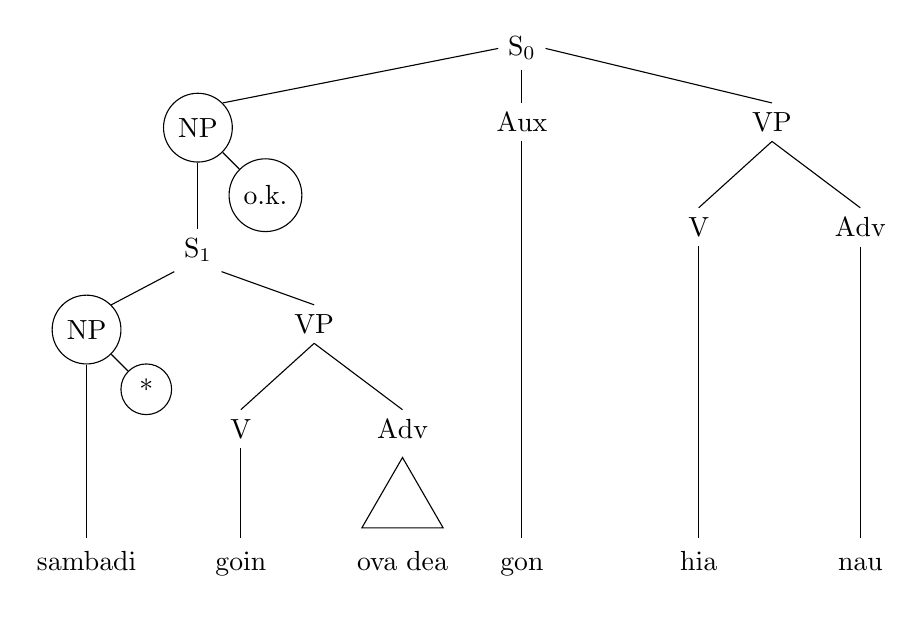
\begin{tikzpicture}[baseline]
	% Draw the nodes
	\node at (0,0) (1S) {S$_0$};
	% Level 2
	\node [below left=\baselineskip and 35mm of 1S, circle, draw] (2NP) {NP};
	\node [below right=\baselineskip and 25mm of 1S] (2VP) {VP};
	\node [below=\baselineskip of 1S] (2Aux) {Aux};
	% Sublevel of 2: "ok"
	\node [below right=3mm of 2NP, circle, draw] (2ok) {o.k.}; 
	% Level 3
	\node [below=2\baselineskip of 2NP] (3S) {S$_1$};
	\node [below left=2\baselineskip and 3mm of 2VP] (3V) {V};
	\node [below right=2\baselineskip and 3mm of 2VP] (3Adv) {Adv};
	% Level 4
	\node [below left=\baselineskip and 8mm of 3S, circle, draw] (4NP) {NP};
	\node [below right=\baselineskip and 8mm of 3S] (4VP) {VP};
	%Sublevel of 4: "*"
	\node [below right=3mm of 4NP, circle, draw] (4*) {*}; 
	% Level 5
	\node [below left=2\baselineskip and 3mm of 4VP] (5V) {V};
	\node [below right=2\baselineskip and 3mm of 4VP] (5Adv) {Adv};
	% Level 6
	% Polygon
	\node [below=1mm of 5Adv, regular polygon, regular polygon sides=3, draw, inner sep=6pt] (6polygon) {};
	\node [on grid, below=1\baselineskip of 6polygon.base, baseline] (6ovadea) {\strut ova dea}; 
	
	\path let \p1 = (5V),  \p2 = (6ovadea) in node at (\x1,\y2) (6goin) {\strut goin};
	\path let \p1 = (4NP),  \p2 = (6ovadea) in node at (\x1,\y2) (6sambadi) {\strut sambadi};
	\path [on grid] let \p1 = (2Aux),  \p2 = (6ovadea) in node at (\x1,\y2) (6gon) {\strut gon};
	\path let \p1 = (3V),  \p2 = (6ovadea) in node at (\x1,\y2) (6hia) {\strut hia};
	\path let \p1 = (3Adv),  \p2 = (6ovadea) in node at (\x1,\y2) (6nau) {\strut nau};
	
	% Draw the paths between nodes
	\draw (node cs:name=1S, anchor=west) -- (node cs:name=2NP, anchor=north east);
	\draw (node cs:name=1S, anchor=east) -- (node cs:name=2VP, anchor=north);
	\draw (node cs:name=1S, anchor=south) -- (node cs:name=2Aux, anchor=north);
	\draw (node cs:name=2NP, anchor=south east) -- (node cs:name=2ok, anchor=north west);
	\draw (node cs:name=2NP, anchor=south) -- (node cs:name=3S);
	\draw (node cs:name=2VP, anchor=south) -- (node cs:name=3V, anchor=north);
	\draw (node cs:name=2VP, anchor=south) -- (node cs:name=3Adv, anchor=north);
	\draw (node cs:name=3S, anchor=south west) -- (node cs:name=4NP, anchor=north east);
	\draw (node cs:name=3S, anchor=south east) -- (node cs:name=4VP, anchor=north);
	\draw (node cs:name=4NP, anchor=south east) -- (node cs:name=4*, anchor=north west); 
	\draw (node cs:name=4VP, anchor=south) -- (node cs:name=5V, anchor=north);
	\draw (node cs:name=4VP, anchor=south) -- (node cs:name=5Adv, anchor=north);
	\draw (node cs:name=4NP, anchor=south) -- (node cs:name=6sambadi);
	\draw (node cs:name=5V, anchor=south) -- (node cs:name=6goin);
	\draw (node cs:name=2Aux, anchor=south) -- (node cs:name=6gon);
	\draw (node cs:name=3V, anchor=south) -- (node cs:name=6hia);
	\draw (node cs:name=3Adv, anchor=south) -- (node cs:name=6nau);
	
	\end{tikzpicture}
}
}
\end{exe}
%\originalpage{37}

\noindent If S\textsubscript{1} constituted an independent sentence, then the rule of subject\-copying would place the appropriate pronoun immediately to the right of the NP marked with an asterisk to yield \textit{sambadi dei goin ova dea}. However, when S\textsubscript{1} is embedded in S\textsubscript{0}, the higher-circled NP node must have the pronoun adjoined to it in order to yield \REF{ex:79}, rather than the ungrammatical \REF{ex:80}.

\citet{Chomsky1964} proposed a universal principle termed the ``A-over-A principle''\is{A-over-A principle}, which states that if a major category, such as NP, is directly dominated by the same major category, then any rule that would normally apply to the lower category node could apply only to the higher node. Although the principle as there formulated has not been widely accepted (cf. \citealt{Ross1967}), similar phenomena have been observed in a number of languages, and something resembling such a principle must still be regarded as a likely formal universal. Formal universals must be regarded part of the innate equipment of the species, and HCE speakers, however they may have arrived at the A-over-A principle\is{A-over-A principle}, cannot have done so as a result of experience.

In the first place, no sentences involving both relativization and subject-copying are found in pre-1920 arrivals, and therefore the varying distribution of copies in relative and nonrelative sentences cannot have been acquired from HPE speakers. The differences from English are obvious: sentences like  \REF{ex:75} and  \REF{ex:79} would be ungramma\-tical even in those so-called ``substandard'' dialects of English which permit subject-copying and/or deletion of relative pronouns in subject position. No substrate language combines similar modes of relativization and focusing; therefore, none of them could have pro\-vided relevant evidence. Moreover, in this case we have much clearer proof than before that the current of innovation ran from HCE back into HPE, rather than vice versa.

Among later immigrants, there was just one (arrival date 1930) who attempted complex sentences such as \REF{ex:79}. Although he some\-times got them right, he would, with equal frequency, produce sen\-tences with two copies, as in \REF{ex:81}, or no copies, as in \REF{ex:82}:

\ea\label{ex:84}
awl diz bigshat pipl dei gat plenti mani dei no kea\\
\glt `All these big shots who have plenty of money don't care' 
\z

\ea\label{ex:85} 
sam kam autsaid kam mo was\\
\glt `Some who come out (of jail) become worse'
\z

\noindent These sentences are of course ungrammatical in HCE, and no locally-born speaker would have produced them. But they are just the kind of vague approximations that are made by foreign-language learners when they try to apply a new and imperfectly-acquired rule. Indeed, HCE, once established, was just that -- a new foreign language -- and joined earlier versions of HPE as a part of the input to immigrant speakers who arrived in Hawaii after 1920.\\\\


We have now surveyed five quite distinct aspects of HCE gram\-mar and found in each of them dear innovations by the earliest HCE
%\originalpage{38}
speakers; developments in the grammar which can have owed little or nothing to HPE, to English, or to any of the substrate languages involved. We may briefly review those developments by presenting a more formal summary in terms of the grammatical rules involved, showing first the HPE rules -- if HPE can be said to have rules or a grammar of its own; I think that HPE would really have to have an analysis like that proposed by \citet{Silverstein1972} for Chinook Jargon, in which the pidgin forms would be produced by extensions and modifications of the HPE speakers' original native languages -- and then the HCE rules for each of the five areas.

With regard to basic sentence-structure and movement rules, HPE would have the following phrase-structure (PS) rules: 

\ea\label{ex:86}
S → $\left\{\begin{array}{lcr} \text{NP} & \text{V} & \text{(NP)}\\\text{NP} & \text{(NP)} & \text{V}\\\text{V} & \text{NP} & \end{array}\right\} $ 
\z

%\originalpage{39}

\noindent HPE would have no movement rules. HCE, on the other hand, would have the following PS rules:

\ea\label{ex:87}
S → NP Aux VP
\z

\ea\label{ex:88}
VP → V (NP) (PP)
\z

\noindent and in addition the following movement rules:

\ea\label{ex:89}
\begin{tabular}[t]{lccr}
SD: & NP & VP & \\
& 1 & 2 & → \\
SC: & 2 & 1 & \\
\end{tabular}
\z
\ea\label{ex:90}
\begin{tabular}[t]{lccrr}
	SD: & X & V & NP & \\
	& 1 & 2 & 3 &  → \\
	SC: & 3 & 1 & 2 & \\
\end{tabular}
\z

For the second area, involving articles\is{articles}, HPE, if it had any rule at all, would have something like \REF{ex:91}: 

\ea\label{ex:91}
NP → $\left\{\begin{array}{l} \text{(da)}\\ \text{(wan)} \end{array}\right\} $ N
\z

\noindent There would be no rule that would determine the circumstances under which \textit{da}, \textit{wan}, or {\O} would be generated. HCE, on the other hand, would have the following rule (I will ignore determiners other than articles\is{articles}): 

\ea\label{ex:92}
NP → Art N
\z

\ea\label{ex:93}
Art → $\left\{\begin{array}{l} \text{Definite} \\ \text{Nondefinite} \\ \text{Nonspecific}\end{array}\right\}$
\z

\ea\label{ex:94}
{\rm Definite}  → da
\z

\ea\label{ex:95}
{\rm Nondefinite} → wan
\z

\ea\label{ex:96}
{\rm Nonspecific} → \O
\z

For the third area, involving \textit{stei} and other auxiliaries, it is not clear what rules, if any, HPE would have -- possibly a rule such as \REF{ex:97}, which would also account for the fact that some auxiliaries, such as \textit{kaen}, may function as main verbs, as in \textit{no kaen} `(You) can't (do it)'/ `It's impossible':

\ea\label{ex:97}
V → (V) V
\z

\noindent HCE, however, would have \REF{ex:87}, plus the following PS rules:

\ea\label{ex:98}
 Aux → (Tense) (Modal) (Aspect)
\z

\ea\label{ex:99}
 Tense → Anterior
\z
\exewidth{(234)}

\ea\label{ex:100}
 Modal → \ldots~Irrealis \ldots
\z

\ea\label{ex:101}
 Aspect → Nonpunctual
\z

\ea\label{ex:102}
 {\rm Anterior} → \textit{bin}
\z

\ea\label{ex:103}
 {\rm Irrealis} → \textit{go}
\z

\ea\label{ex:104}
 {\rm Nonpunctual} → \textit{stei}
\z

%\originalpage{40}

For the fourth area, involving \textit{fo}, \textit{go}, and sentential comple\-ments, HPE would have no rules. HCE would possibly have something like the following PS rule (but see \chapref{ch:2} on the status of complementizers in creoles generally):

\ea\label{ex:105}
NP → (COMP) S 
\z

\ea\label{ex:106}
 COMP → $\left\{\begin{array}{l}\text{Realized}\\\text{Unrealized}\end{array}\right\}$
\z

\ea\label{ex:107}
 {\rm Realized} → \textit{go}
\z

\ea\label{ex:108}
{\rm Unrealized} → \textit{fo}
\z

\noindent In addition, HCE would require something analogous to (but probably not identical with) the English rule of equi-deletion.

Finally, for the fifth area, involving relativization, subject-copying, and their interaction, we might need a rule for Filipino speakers which would modify \REF{ex:97} to something like \REF{ex:109}:

\ea\label{ex:109}
 V → $\left\{\begin{array}{l}\text{(V)\; V}\\\text{({\it i})\; V}\\\text{Pred}\end{array}\right\}$
\z

\noindent (All but the later HCE-influenced HPE speakers realize the copy, if indeed for them it is a copy -- it is more likely a marker of a particular predicate type -- as an invariant \textit{i}, i.e., in contradistinction to the HCE rule, subject features such as \textit{plural} or \textit{feminine} are not copied onto it.) A few speakers might have, in addition, a rule for relativization that would simply replace NP by S. HCE speakers would have a well-established rule:

\ea\label{ex:110}
 NP → S
\z

\noindent In addition, they would have the following transformational rule:

%{\textbackslash}

% % PIDGIN INTO CREOLE 41

\ea\label{ex:111}
\begin{tabular}{lllcr}
	SD: & & NP & VP\\
	    & \multicolumn{2}{l}{$\left[\begin{array}{l}\alpha\; \text{number}\\\beta\; \text{gender}\end{array}\right]$} & & \\
	    & & \hspaceThis{$\alpha$}1 & 2 & →\\
	SC: & &\hspaceThis{$\alpha$}1 + pro & & 2\\
	    & &\multicolumn{3}{l}{$\hspaceThis{1 +}\left[\begin{array}{l}\alpha\; \text{number}\\\beta\; \text{gender}\end{array}\right]$}\\
\end{tabular}
\z

\noindent The A-over-A principle\is{A-over-A principle}, or whatever general constraint governs the subject-copying rule in relativized sentences, would not need to be separately stated in the HCE grammar since it would presumably be a universal.

All that remains for us is to ask how these quite substantial innovations could have been produced. There would seem to be only two logically possible alternatives. They could have been produced by some kind of general problem-solving device such as might be applied in any field of human behavior where the required human institutions were lacking -- much as survivors of a shipwreck or an atomic holocaust might reconstruct government, laws, and other social institutions. Or they might have been produced by the operation of innate faculties genetically programmed to provide at least the basis for an adequate human language.

If Hawaii were the only place where people had been faced with the problem of reconstructing human language, it would be impossible to decide between these alternatives. However, Hawaii is far from unique. There are a number of creole languages in other parts of the globe, but produced under very similar circumstances, several of which have been described well enough to make comparison possible. It is true that in these cases we do not have the antecedent pidgin for comparative purposes,\footnote{\citet{Alleyne1979} uses this fact to argue that there never were antecedent pidgins -- if there had been, he claims, they should have left traces in contemporary creoles, but he denies the existence of such traces. This argument will be dealt with further in \chapref{ch:2}. Meanwhile, the reader may well wonder how much pidgin structure one could legitimately expect to be left in creoles, given the relation\-ship between the rules of HPE and HCE illustrated in \REF{ex:86}--\REF{ex:111} above.} but we shall see that there are still some oblique indications of antecedent structure. In any case, it is difficult to see, given the rapidity with which creoles arose, how those antecedent pidgins could have developed any further than Hawaii's did.

%\originalpage{42}

Now, of the two alternatives stated above, each would seem to make different predictions about the general nature of creoles. If some general problem-solving device were at work, we would not expect that in every different circumstance it would reach the same set of conclusions. There are any number of possible solutions to the struc\-tural and communicative problems that language poses, as the very diversity of the world's languages shows, and we would expect to find that, given the differences in geographical region, culture, contributing languages, and so on, each group faced with the task of reconstructing language would arrive at quite different solutions. Indeed: unless I am mistaken, orthodox generativists, even while believing in an innate language faculty, might predict the same result since their theory assigns to that faculty nothing more than those formal and substantive universals which are reflected in all languages. Thus, they could pre\-dict no more of a creole than that it should not violate any universal constraint.

However, if all creoles could be shown to exhibit an identity far beyond the scope of chance, this would constitute strong evidence that some genetic program common to all members of the species was decisively shaping the result.

%{\textbackslash}
  
 

%%%%%%%%%%%%%%%%%%%%%%%%%%%%%%%%%%%%%%%%%%%%%%%%%%%%
%%%                                              %%%
%%%             Backmatter                       %%%
%%%                                              %%%
%%%%%%%%%%%%%%%%%%%%%%%%%%%%%%%%%%%%%%%%%%%%%%%%%%%%

% There is normally no need to change the backmatter section
\backmatter
\phantomsection%this allows hyperlink in ToC to work
%\addcontentsline{toc}{chapter}{References}
\printbibliography[heading=references]   
   
\phantomsection 
\addcontentsline{toc}{chapter}{Index} 
\addcontentsline{toc}{section}{Name index}
\ohead{Name index} 
\printindex 
  
\phantomsection 
\addcontentsline{toc}{section}{Language index}
\ohead{Language index} 
\printindex[lan] 
  
\phantomsection 
\addcontentsline{toc}{section}{Subject index}
\ohead{Subject index} 
\printindex[sbj]

\end{document} 

% you can create your book by running
% xelatex lsp-skeleton.tex
%
% you can also try a simple 
% make
% on the commandline
